\documentclass{beamer}
\usepackage{../common_slides}
\usepackage{pdfpages}

\title{CS287: Statistical Natural Language Processing}

\newenvironment{changemargin}{%
\begin{list}{}{%
\vspace{-1cm}
\setlength{\topsep}{0pt}%
\setlength{\leftmargin}{-1cm}%
\setlength{\rightmargin}{-1cm}%
\setlength{\listparindent}{\parindent}%
\setlength{\itemindent}{\parindent}%
\setlength{\parsep}{\parskip}%
}%
\item[]}{\end{list}}

\author{Alexander Rush}
\begin{document}


\begin{frame}
  \titlepage
\end{frame}

\section{Applications}

{
\setbeamercolor{background canvas}{bg=}
\includepdf[pages=3-4]{slides.pdf}
}

\begin{frame}
  \begin{center}
    \includegraphics[width=5cm]{siri}
  \end{center}
\end{frame}

\begin{frame}
  \begin{changemargin}
  \begin{center}
    \includegraphics[height=1.1\textheight]{echo}
  \end{center}
  \end{changemargin}
\end{frame}


\begin{frame}
  \begin{center}
    \includegraphics[height=\textheight]{abelincoln}
  \end{center}
\end{frame}

% \begin{frame}{Automatic Translation}
%   \begin{center}
%     \includegraphics{translate}
%   \end{center}
% \end{frame}

\section{Scientific Challenges}

\begin{frame}{Foundational Challenge: Turing Test}
  \begin{quote}
    Q: Please write me a sonnet on the subject of the Forth Bridge.

    A : Count me out on this one. I never could write poetry.

    Q: Add 34957 to 70764.
    
    A: (Pause about 30 seconds and then give as answer) 105621.
    
    Q: Do you play chess?
    
    A: Yes.
    
    Q: I have K at my K1, and no other pieces. You have only K at K6 and R at R1. It is your move. What do you play?

    A: (After a pause of 15 seconds) R-R8 mate.
      {\normalfont - Turing (1950)}
  \end{quote}

\end{frame}

\begin{frame}{(1) Lexicons and Lexical Semantics}
  \textbf{Zipf' Law (1935,1949):}
  \begin{quote}
    The frequency of any word is inversely proportional to its rank in the frequency table.
  \end{quote}


     \begin{center}
       \includegraphics[width=0.8\textwidth]{../notebooks/zipf}         
     \end{center}
% \begin{itemize}
  % \item I.e. it is common to use rare words. 
  % \item Central issue in NLP is dealing cleverly with rare words. 
  % \end{itemize}
\end{frame}


\begin{frame}{(2) Structure and Probabilistic Modeling }
  \textbf{The Shannon Game (Shannon and Weaver, 1949):}
  \begin{quote}
    Given the last $n$ words, can we predict the next one?
  \end{quote} 
  

  \texttt{The pin-tailed snipe (Gallinago stenura) is a small stocky wader. It breeds in northern Russia and migrates to spend the \_\_ } 


  \begin{itemize}
  \item Probabilistic models have become very effective at this task.
  \item Crucial for speech recognition (Jelinek), OCR, automatic translations, etc. 
  \end{itemize}



\end{frame}

\begin{frame}{(3) Compositionality of Syntax and Semantics}
  \begin{quote}
    Probabilistic models give no insight into some of the basic
    problems of syntactic structure  {\normalfont - Chomsky (1956)}
  \end{quote}
  \begin{center}
    \includegraphics[width=10cm]{syntaxsem}
  \end{center}
\end{frame}


\begin{frame}{(4) Document Structure and Discourse}
  \begin{quote}
    Language is not merely a bag-of-words but a tool with particular
    properties  { - \normalfont Harris (1954)}
  \end{quote}
  \begin{center}
    \includegraphics[width=\textwidth]{cort}
  \end{center}
\end{frame}

\begin{frame}{(5) Knowledge and Reasoning Beyond the Text}
\begin{quote}
It is based on the belief that in modeling language understanding, we must deal in an integrated way with all of the aspects of language — syntax, semantics, and inference. {- \normalfont Winograd (1972) }  
\end{quote}


\texttt{The city councilmen refused the demonstrators a permit because they [feared/advocated] violence.}


\begin{itemize}
\item Recently (2011) posed as a challenge for testing commonsense reasoning.  

\end{itemize}
\end{frame}


\section{Deep Learning for Natural Language Processing}

\begin{frame}{Deep Learning and NLP}
  \begin{itemize}
  \item Presentation-based on Chris Manning's ``Computational Linguistics and Deep Learning'' (2016) published in \textit{Computational Linguistics} 
  \end{itemize}

  \begin{quote}
    Deep Learning waved have lapped at the shores of computational linguistics for several years now, but 2015 seems like the year when the full force of the tsunami hit major NLP conferences. {\normalfont - Chris Manning}
  \end{quote}

\end{frame}

\begin{frame}{NLP as a Challenge for Machine Learning}

  \begin{quote}
    I'd use the billion dollars to build a NASA-size program focusing
    on natural langauge processing in all of its glory (semantics,
    pragmatics, etc.) ... Intellectually I think that NLP is
    fascinating, allowing us to focus on highly structure inference
    programs, on issues that go to the core of `what is thought` but
    remain eminently practical, and on a technology that surely would
    make the world a better place'' {\normalfont - Jordan
      (2014)}
  \end{quote}
\end{frame}

\begin{frame}{NLP as a Challenge for Deep Learning}

  \begin{quote}
  The next big step for Deep Learning is natural language
  understanding, which aims to give machines the power to understand
  not just individual words but entire sentence and paragraphs. {\normalfont - Bengio }
  \end{quote}
\end{frame}

\begin{frame}{What are they referring to?}
  Recent advances in,
  \begin{itemize}
  \item Speech Recognition 
  \item Language Modeling 
  \item Machine Translation
  \item Question Answering
  \item many other tasks.
  \end{itemize}

  \pause 
  Still,
  \begin{quote}
    Problems in higher-level language processing have not seen the dramatic error-rate reductions from deep learning 
    that have been seen in speech recognition and object recognition in vision.
  \end{quote}

\end{frame}


\begin{frame}{Object Recognition}
  \begin{center}
    \includegraphics[width=\textwidth]{mylenet}
  \end{center}
\end{frame}

\begin{frame}
  \vspace{-0.25cm}

  \begin{center}
    \includegraphics[height=\textheight]{filters}
  \end{center}
\end{frame}


\begin{frame}{Image Captioning}
  \begin{center}
    \includegraphics[width=\textwidth]{good}
    \caption{Xu et al (2015)}
  \end{center}
\end{frame}

\begin{frame}{Central Aspects of Deep Learning for NLP}
  \begin{enumerate}
  \item Learn the features representations of language.
    \pause
    \air 

  \item Construct higher-level structure in a latent manner
    \pause
    
    \air

  \item Train systems completely end-to-end.
  \end{enumerate}
\end{frame}

\begin{frame}
  \vspace{-5cm}
  
  \hspace*{-2cm}
  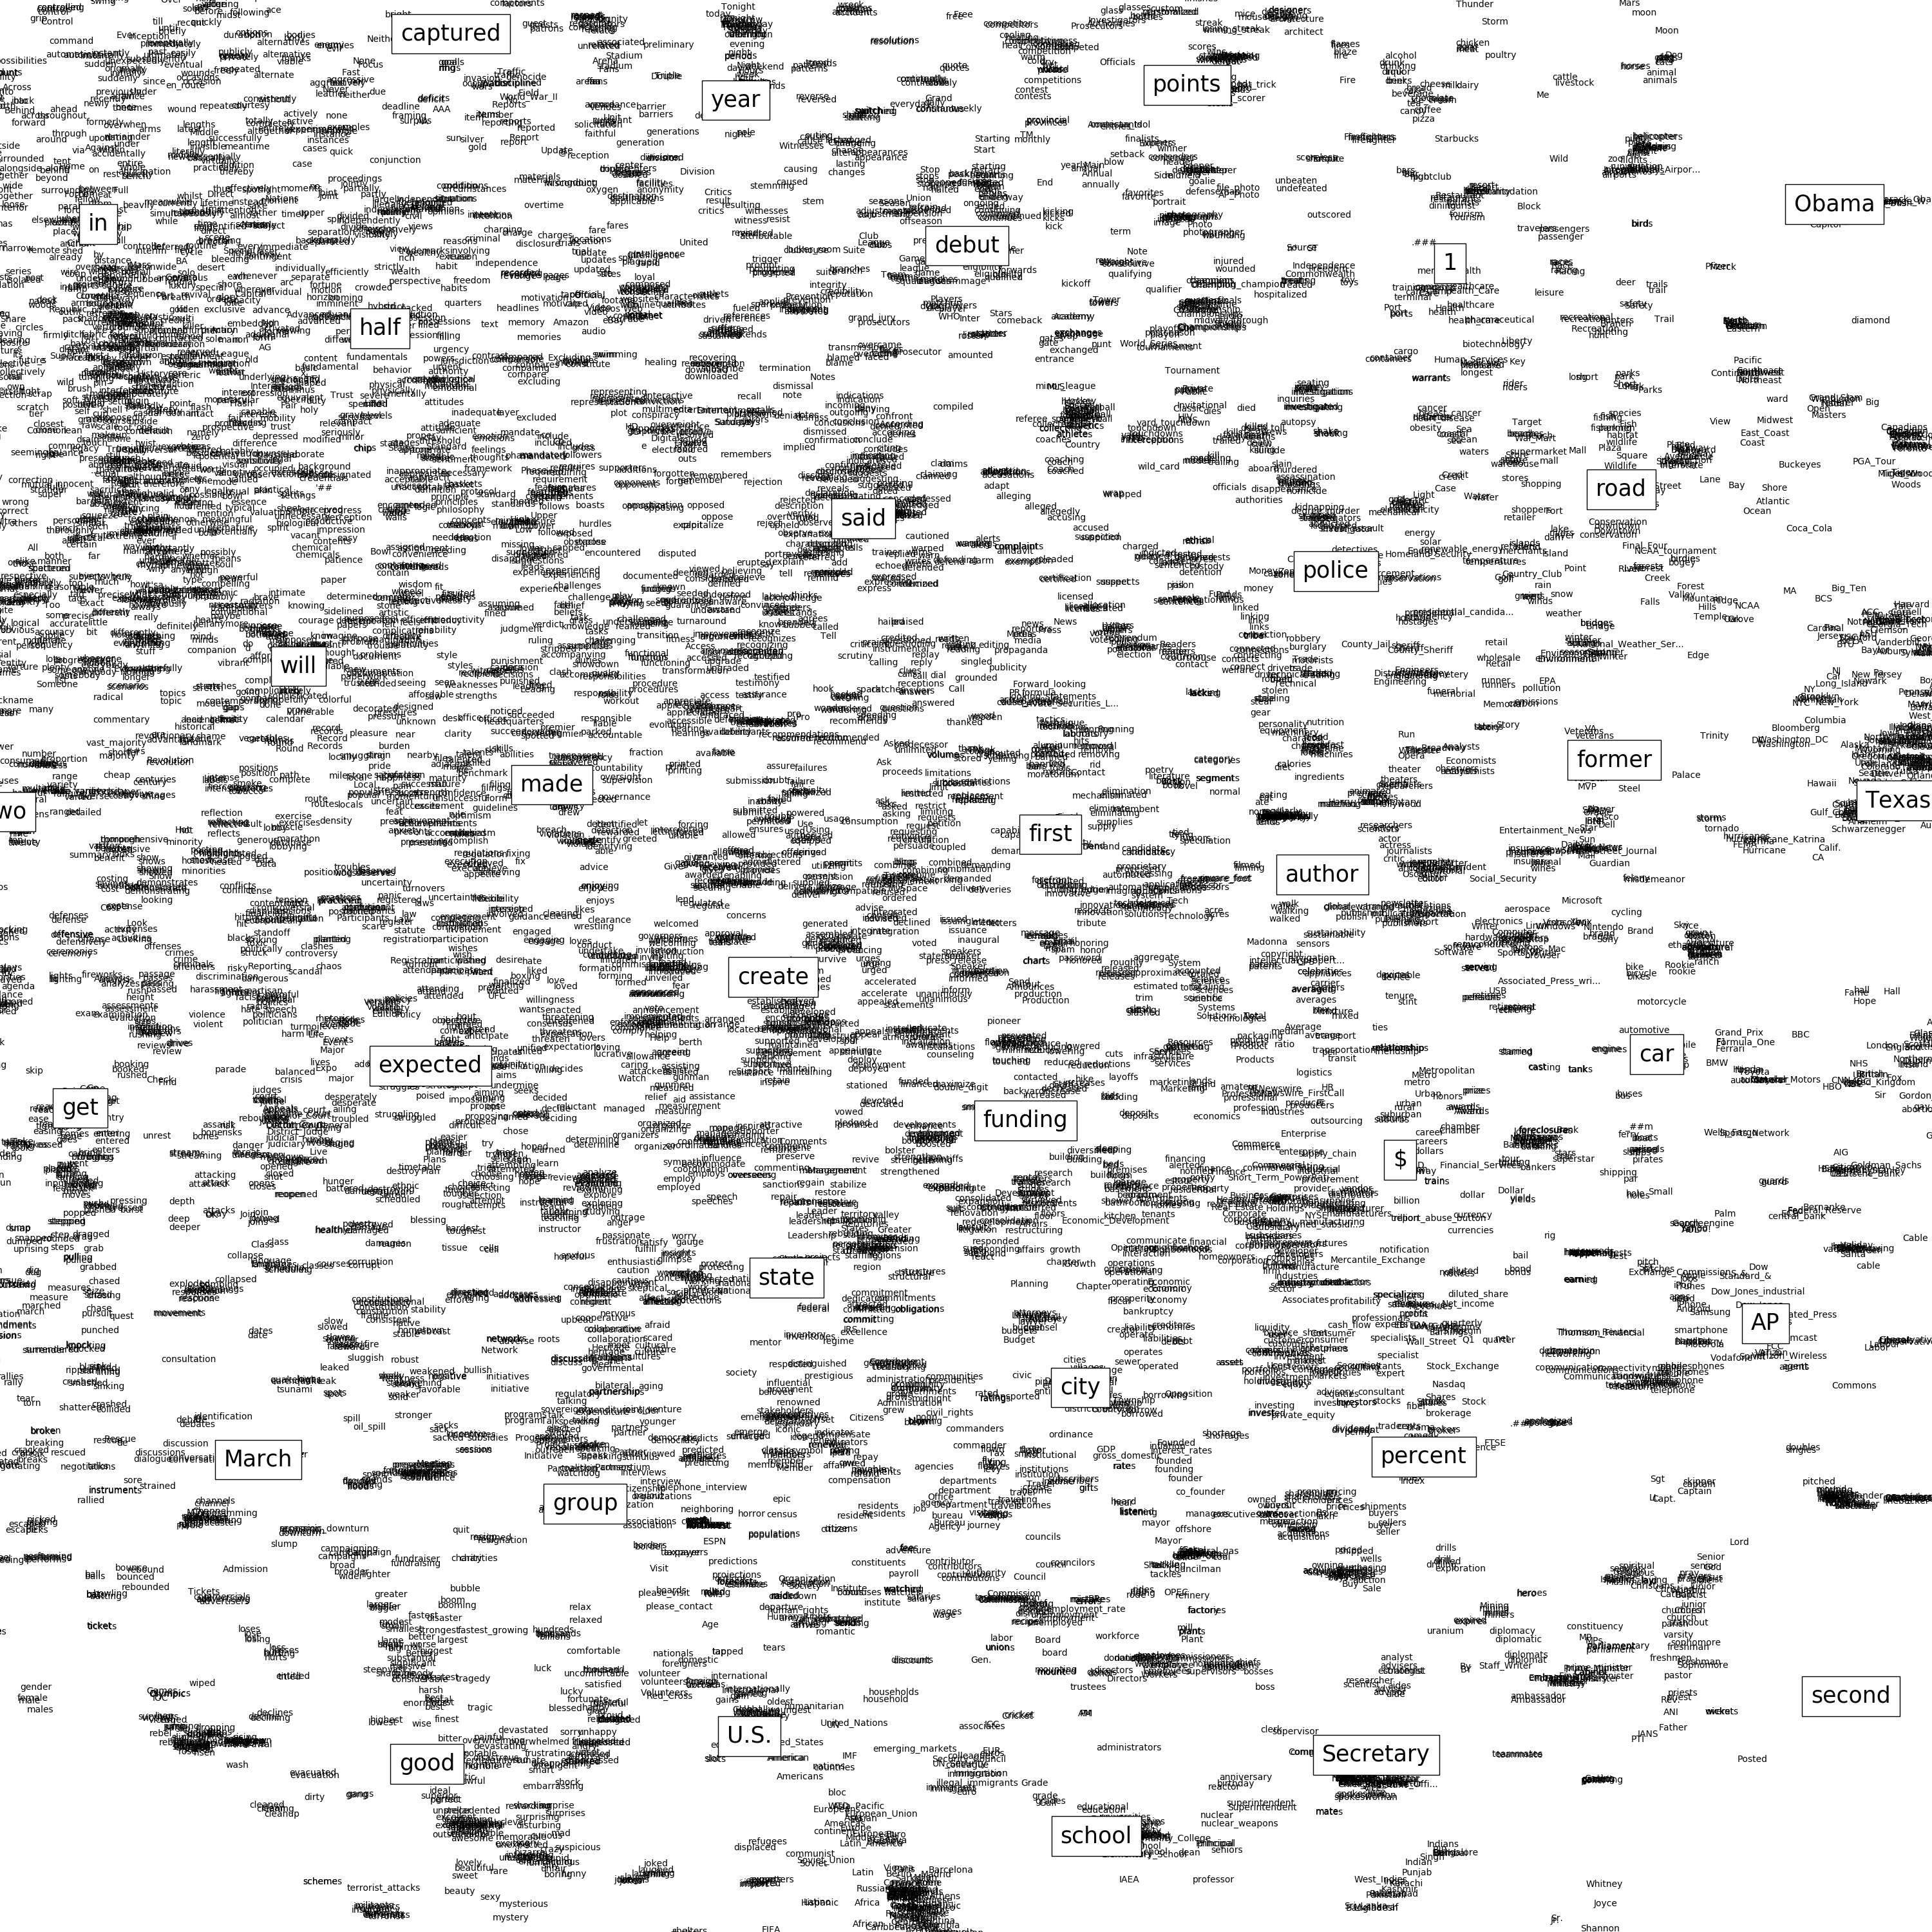
\includegraphics[width=1.5\textwidth]{../notebooks/graph}
\end{frame}

\begin{frame}
  \begin{center}
    \includegraphics[width=1\textwidth]{compare}
  \end{center}
\end{frame}


\begin{frame}{LSTM}
  \begin{center}
    \includegraphics[width=\textwidth]{LSTM3-chain}
  \end{center}
\end{frame}


\begin{frame}
  \begin{center}
    \includegraphics[height=\textheight]{../latex3}
  \end{center}
\end{frame}


\begin{frame}
  \begin{center}
    \includegraphics[width=\textwidth]{lstm1}
  \end{center}
\end{frame}

\begin{frame}{GPU Processing}

  \begin{itemize}
  \item Neural Networks are remarkably parallel-izable. 
  \end{itemize}

  GPU Implementation of a variant of HW1  

  \begin{center}
    \begin{tabular}{lll}
      \toprule
      & non-GPU & GPU\\
      \midrule
      per epoch& 2475s & 54.0 s \\
      per batch & 787ms & 15.6 ms\\
      \bottomrule
    \end{tabular}
  \end{center}
\end{frame}

\begin{frame}{(1) Compositional Structures?}
  \begin{center}
    \includegraphics[width=\textwidth]{sentiment}
  \end{center}
\end{frame}

\begin{frame}{(2) Understanding Text?}
  \includegraphics[width=\textwidth]{cell}
\end{frame}


\begin{frame}{(3) Language and Thought?}
  \begin{itemize}
  \item Do these methods tell us anything about core nature of language?
    \air 

  \item Do they inform psychology or cognitive problems?
  \end{itemize}
\end{frame}

\section{This Class}

\begin{frame}{This Semester}
  Deep Learning for Natural Language Processing

  \begin{itemize}
  \item Primarily a lecture course. 
    \air 

  \item Topics and papers distributed throughout.
    \air

  \item Main Goal: Educate researchers in NLP
  \end{itemize}
\end{frame}

\begin{frame}{Background}
  \begin{itemize}
  \item Some college-level Machine Learning course
  \item Practical programming experience
  \item Interest in applied experimental research (not a theory course)
  \end{itemize}
\end{frame}

\begin{frame}{Audience}
  Take this class to...
  \begin{itemize}
  \item understand about cutting-edge methods in the area. 
  \item replicate many important recent results 
  \item apply machine learning to relevant, interesting problems
  \end{itemize}
  \pause 

  Do not take this class to...
  \begin{itemize}
  \item get experience with common NLP tools (NLTK, CoreNLP, etc.)
  \item build a system for your (non-NLP) startup
  \item learn much about modern Linguistics
  \end{itemize}
\end{frame}

\begin{frame}{Topics}

  \begin{enumerate}
  \item Machine Learning for Text
    \pause
    \air
  \item Feed-Forward Neural Networks
    \pause
    \air 
  \item Language Modeling and Word Embeddings 
    \pause
    \air
  \item Recurrent Neural Networks
    \pause
    \air
  \item Conditional Random Fields and Structured Prediction
  \end{enumerate}
\end{frame}

\begin{frame}{Homeworks}
  Each homework will require you to replicate a research result,

  \begin{itemize}
  \item Text Classification
  \item Sentence Tagging
  \item Language Modeling (1)
  \item Language Modeling (2) (LSTMs)
  \item Name-Entity Recognition (CRFs)
  \end{itemize}

\end{frame}

\begin{frame}{Programming}
  Assignments use,
  \begin{itemize}
  \item Python for text processing and visualization
  \item Lua/Torch for neural networks

  \begin{center}
    \includegraphics[width=4cm]{torch}
  \end{center}

   \item First section on Fri. will be introduction.
  \end{itemize}
\end{frame}


\begin{frame}{Applications}
  Lectures on NLP applications
  
  \begin{itemize}
  \item Language Modeling
    \air 
  \item Coreference and Pronoun Anaphora
    \air

  \item Neural Machine Translation
    \air 

  \item Syntactic Parsing

  \end{itemize}
\end{frame}


\begin{frame}{Final Project}
  \begin{itemize}
  \item Empirical project done in teams
    \air 

  \item Research-level project on current topics
    \air

  \item Expect top projects to be conference submissions.
  \end{itemize}
\end{frame}

\begin{frame}{Project Ideas}
  Projects we work on,
  \begin{itemize}
  \item Morphology in language modeling
  \item In-Document Coreference
  \item Surface ordering of words in a sentence. 
  \item Question-Answering in Text
  \end{itemize}
\end{frame}


\begin{frame}{Project Ideas}
  Projects we work on $\ldots$
  \begin{itemize}
  \item Morphology in language modeling
  \item In-Document Coreference
  \item Surface ordering of words in a sentence. 
  \item Question-Answering in Text
  \end{itemize}
\end{frame}


\begin{frame}{Project Ideas}
  Projects to consider $\ldots$
  \begin{itemize}
  \item Information Extraction from Documents
  \item Twitter and Social Network Modeling
  \item Visualization of NLP networks
  \item Deep-Reinforcement Learning and Languages
  \end{itemize}
\end{frame}

\begin{frame}{}
  \begin{center}
    \includegraphics[height=\textheight]{minsky}
  \end{center}
  \notes{- Two undergraduate students Marvin Minsky at Harvard in 1950, build the first neural network computer the SNARC (3000 Vacuum tubes and a surplus autopilot mechanism form a B-24 bomber)
- von neumann ``If it isn't now it will be someday''}
\end{frame}


\end{document}